\documentclass[]{paper}
\usepackage{}

% type user-defined commands here
\usepackage{graphicx}
\usepackage{color}
\usepackage{url}
\usepackage{fullpage}
\usepackage{caption}
\usepackage{subcaption}
% type user-defined commands here                                                                                                                         
\newif\ifdraft
\drafttrue
\ifdraft
\newcommand{\onote}[1]{ {\textcolor{cyan} { (***Ole: #1) }}}
\newcommand{\terminology}[1]{ {\textcolor{red} {(Terminology used: \textbf{#1}) }}}
\newcommand{\owave}[1]{ {\cyanuwave{#1}}}
\newcommand{\jwave}[1]{ {\reduwave{#1}}}
\newcommand{\alwave}[1]{ {\blueuwave{#1}}}
\newcommand{\jhanote}[1]{ {\textcolor{red} { ***shantenu: #1 }}}
\newcommand{\alnote}[1]{ {\textcolor{green} { ***andreL: #1 }}}
\newcommand{\amnote}[1]{ {\textcolor{blue} { ***andreM: #1 }}}
\newcommand{\smnote}[1]{ {\textcolor{brown} { ***sharath: #1 }}}
\newcommand{\pmnote}[1]{ {\textcolor{brown} { ***Pradeep: #1 }}}
\newcommand{\mrnote}[1]{ {\textcolor{cyan} { ***Melissa: #1 }}}
\newcommand{\note}[1]{ {\textcolor{magenta} { ***Note: #1 }}}
\else
\newcommand{\onote}[1]{}
\newcommand{\terminology}[1]{}
\newcommand{\owave}[1]{#1}
\newcommand{\jwave}[1]{#1}
\newcommand{\alnote}[1]{}
\newcommand{\amnote}[1]{}
\newcommand{\athotanote}[1]{}
\newcommand{\smnote}[1]{}
\newcommand{\pmnote}[1]{}
\newcommand{\jhanote}[1]{}
\newcommand{\mrnote}[1]{}
\newcommand{\note}[1]{}
\fi

\newcommand{\up}{\vspace*{-1em}}
\newcommand{\upp}{\vspace*{-0.5em}}
\newcommand{\pilotmapreduce}{Pilot-MapReduce\xspace}


\begin{document}

\title{FutureGrid 2012 Project Challenge:\\ Using SAGA to build Scalable Dynamic Distributed Applications}
%\title{FutureGrid 2012 Student Project Challenge} 
\author{Pradeep Kumar Mantha 
  \and Sivakarthik Natesan 
  \and Melissa Romanus \\
  \and Sai Saripalli 
  \and Ashley Zebrowski 
  \and \large{Faculty Advisor: Shantenu Jha}\\
  }

\date{May 15th, 2012}
\maketitle

% \begin{abstract}
% \end{abstract}

\section{Introduction}

% The development of scalable and applications presents a formidable research challenge.  

There are multiple challenges in the effective design and implementations of scalable distributed applications and infrastructure: the spectrum of challenges range from managing the heterogeneity inherent in distributed systems on the one hand to the lack of well established programming models to support distributed applications. In addition there do not exist well defined set of base capabilities or unifying abstractions needed to reason about how, when and where to distribute applications. Against this backdrop, the range of distributed cyberinfrastructure (DCI) available to researchers is continually evolving.  Thus, the process of designing and deploying large-scale DCI, as well as developing applications that can effectively utilize them, presents a critical and challenging agenda for domain researchers and CI developers alike.

FutureGrid~\cite{fg} provides students and researchers with new possibilities to engage in science relating to the state-of-the-art in cloud and grid computing.  As student members of the Research in Distributed Cyberinfrastructure and Applications (RADICAL) group, we have taken full advantage of the opportunities that FutureGrid provides.

The students of the RADICAL group have been using SAGA on FutureGrid to address a wide spectrum of challenges: from scalable runtime systems for distributed data-intensive applications (Pilot-MapReduce) to novel dynamic execution modes for traditional HPC applications (Cactus-Spawner) as well as enhanced sampling algorithms (Replica-Exchange).  In addition to flexible and scalable applications, we have used FutureGrid to enhance and extend the capabilities of SAGA.  In this submission we outline how are some of the ways we are using SAGA on FutureGrid resources to build scalable production runtime systems and software whilst pushing the envelope by pursuing exciting new progamming models and possibilities in application space.

% \jhanote{Each section should have the following: Scientific Motivation/objective? How was FutureGrid used? Scientific Results on Futuregrid? Ideally show how this work contributed to Interoperability and scalability}

\section{Pilot-MapReduce}

\jhanote{this needs massive reduction and focus!}

%Scientists in many science disciplines, where enormous amounts of data is generated , e. g. in %the areas of fusion energy, bioinformatics, climate and astronomy, utilize distributed cyber-
%infrastructure to conduct experiments and improve their understanding about the scientific %applications. 

% Scientific Motivation

%Domain scientists face various challenges associated with processing of data at extreme scales, %generated by various data intensive applications on distributed cyberinfrastructures like %FutureGrid. Therefore, an efficient processing of large distributed datasets is required, whilst %deally not introducing fundamentally new programming models or methods. For example, %extending MapReduce - a proven effective programming model for processing large datasets, %to work more effectively on distributed data is desirable. 
%Hadoop is an open-source implementation of MapReduce programming model but is designed %for shared-nothing environments and its performance is affected on a distributed file system.  %On DCI like FutureGrid, we were not able to run Hadoop on multiple clusters due to firewall %issues. MapReduce on distributed data requires effective distributed coordination of %computation (map and reduce) and data, as well as distributed data management (in particular %the transfer of intermediate data units). 

An increasing amount of data that scientific applications need to operate on is distributed. For example, the Earth Science Grid federates data of various climate simulations~\cite{ESG}. Meta-genomic workflows need to process and analyze data generated by various sequencing machines~\cite{Jha:2011fk}; the localization onto a single resource is often not a possibility.
Several options for running Hadoop on distributed data have been proposed~\cite{weissman-mr-11}: (i) in a global Hadoop~\cite{hadoop} setup one central JobTracker and HDFS NameNode is used for managing a distributed set of resources; (ii) in a hierarchical Hadoop setup multiple MapReduce clusters are used: a MapReduce cluster close to the data source for pre-processing data and a central cluster for aggregating the different de-central data sources.

Ref~\cite{weissman-mr-11} shows that a hierarchical Hadoop configuration leads to a better performance than a global Hadoop cluster for high data aggregation applications like WordCount. %  On DCI like we were not able to run global Hadoop on multiple clusters due to firewall issues.
A drawback of hierarchical Hadoop approach is the increased complexity: Hadoop is not designed with respect to a federation of multiple MapReduce clusters. Setting up such a system typically requires a lot of manual effort.

To address these requirements, we design and implement Pilot-MapReduce (PMR)~\cite{pmr-2012} - a flexible, infrastructure-independent runtime environment for MapReduce. PMR is based on Pilot abstractions for both compute (Pilot-Jobs) and data (Pilot-Data)~\cite{pstar-2012}: it utilizes Pilot-Jobs to couple the map phase computation to the nearby source data, and Pilot-Data to move intermediate data using parallel data transfers to the reduce computation phase. Figure ~\ref{fig:mr_arch} depicts the architecture of PMR. 

% PMR Architecture figure.
\begin{figure}[t]
	\begin{subfigure}[b]{0.5\textwidth}
                \centering
                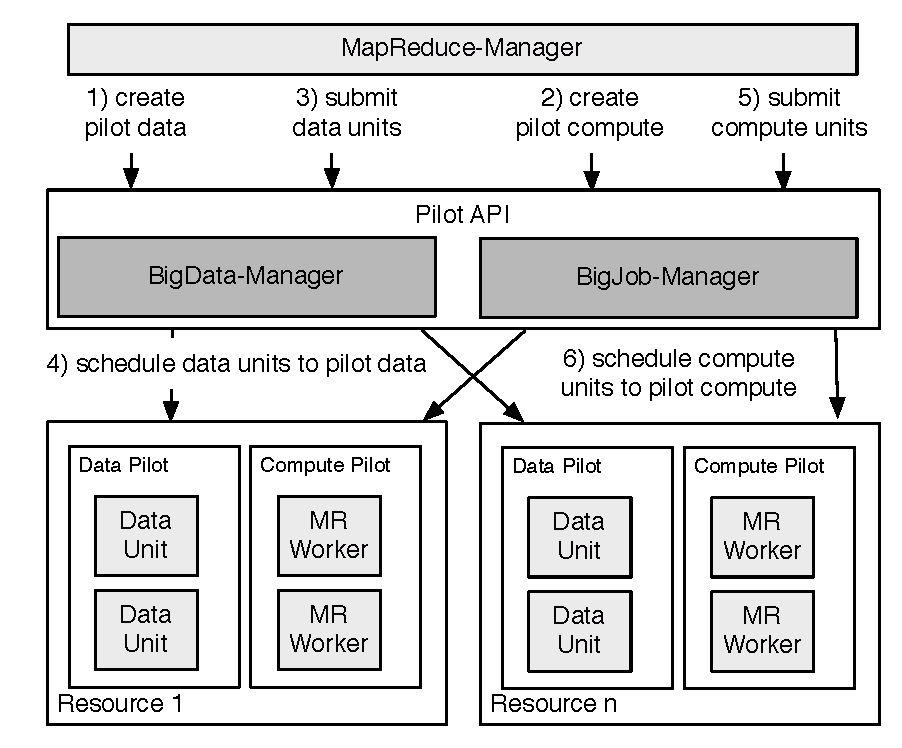
\includegraphics[width=1\textwidth]{figures/mr-arch.pdf}
                \caption{\textbf{Pilot-based MapReduce}}
                \label{fig:mr_arch}
        \end{subfigure}
	\begin{subfigure}[b]{0.5\textwidth}
                \centering
                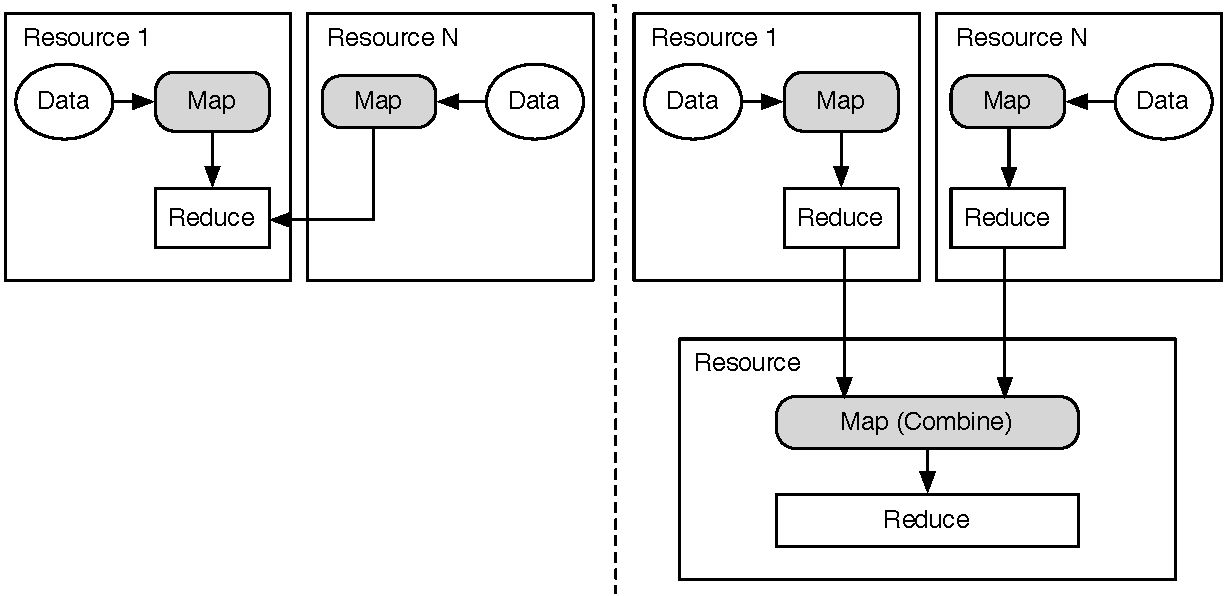
\includegraphics[width=1\textwidth,height=.8\textwidth]{figures/distributed_hierachical.pdf}
                \caption{\textbf{Pilot-MapReduce Deployment Scenarios}}
                \label{fig:mrtop}
        \end{subfigure}

	\caption{ Figure ~\ref{fig:mr_arch} shows the architecture of Pilot-MapReduce, Pilot-Jobs manage the map and reduce compute  units and Pilot-data manage the intermediate data transfer between the map and reduce phase across multiple clusters. Figure ~\ref{fig:mrtop} shows different Pilot-MapReduce Deployment Scenarios- In the distributed scenario (~\ref{fig:mrtop}: left), the mapping tasks are run close to the data; reduced tasks are then run on a single resource. In the hierarchical scenario (~\ref{fig:mrtop}:right) two full MapReduce runs are conducted.  }
	\label{fig:combo_2}

\end{figure}

Pilot-MapReduce supports different distributed MapReduce topologies: (i) local, (ii) distributed and (iii) hierarchical. A local PMR performs all map and reduce computations on a single resource. Figure ~\ref{fig:mrtop} shows options (ii) and (iii): A distributed PMR utilizes multiple resources often to run map tasks close to the data to avoid costly data transfers; the intermediate data is then moved to another resource for running the reduce tasks. ~\cite{pmr-2012}

%topology picture
%\begin{figure}
%	\centering
%	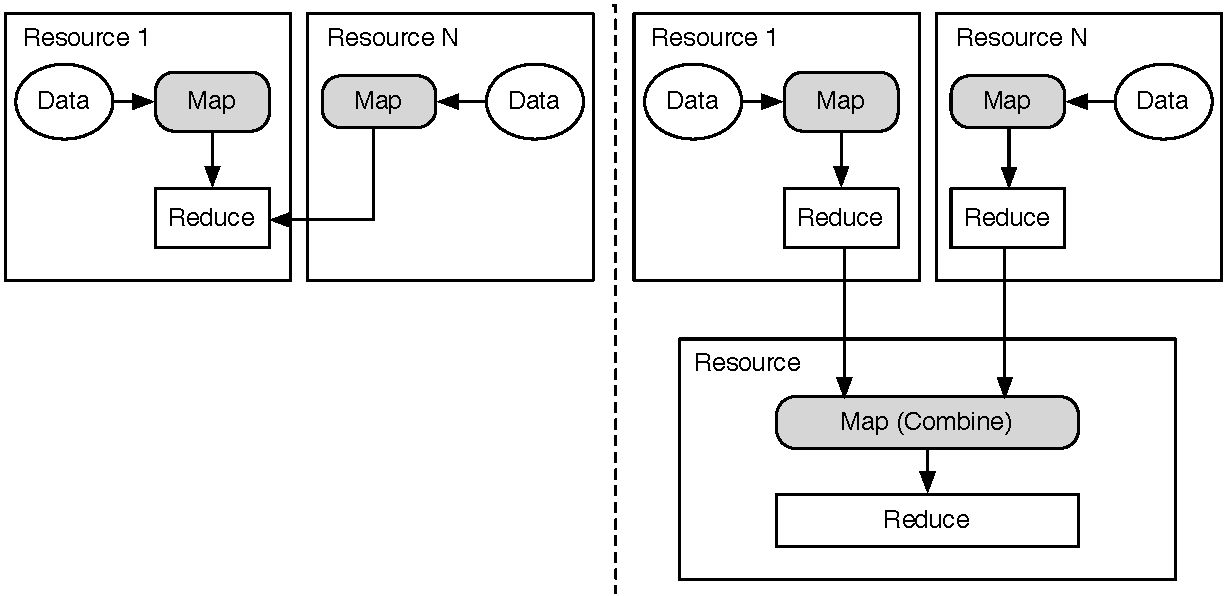
\includegraphics[width=0.40\textwidth]{figures/distributed_hierachical.pdf}
%	\caption{\textbf{Pilot-MapReduce Deployment Scenarios}: In the
%         distributed scenario (left), the mapping tasks are run close
%       to the data; reduced tasks are then run on a single
%        resource. In the hierarchical scenario (right) two full
%         MapReduce runs are
%         conducted. \label{fig:mrtopologies}}
%\end{figure}

%%%%%%%%%%%%%%%%%%%
%End Motivation for PMR
%%%%%%%%%%%%%%%%%%%
%How futuregrid is used.
%%%%%%%%%%%%%%%%%%%
FutureGrid has been an important testbed for the development of Pilot abstractions and PMR.
Our experimental evaluations on FutureGrid show that the \textit{innovative} utilization of Pilot abstractions for compute and data treatment in MapReduce framework, across multiple clusters is promising, and can lower the execution time span of the entire MapReduce execution. To demonstrate the performance, extensibility and scalability of PMR, we utilized FutureGrid resources India, Sierra and Hotel.  We benchmarked PMR against Hadoop using various MapReduce topologies and each experiment is repeated at least three times.

%Scientific results on futuregrid.
%Performance comparision of Hadoop and PMR on FutureGrid.
The \textit{performance} and \textit{scalability} of PMR with distributed data is compared to Hadoop MapReduce using canonical WordCount application on both natural language and random data using different MapReduce topologies.  We utilize two machines, Sierra and Hotel. For all configurations, we use 8 nodes. Table~\ref{tab:data-volumes} summarizes the characteristics of the WordCount application on natural language and random data.

\begin{figure}[t]
	\begin{subfigure}[b]{0.5\textwidth}
                \centering
                \begin{tabular}{|p{1cm}|c|c|c|}
\hline
\textbf{Data Stage}&\textbf{Natural Language}&\textbf{Random Data}\\
\hline
Input  &16\,GB&16\,GB\\
\hline
Inter-mediate &26\,GB&30\,GB\\ 
\hline
Output &20\,MB&30\,GB\\
\hline
\end{tabular}
		
                \caption{}
                \label{tab:data-volumes}
        \end{subfigure}
	\begin{subfigure}[b]{0.5\textwidth}
                \centering
                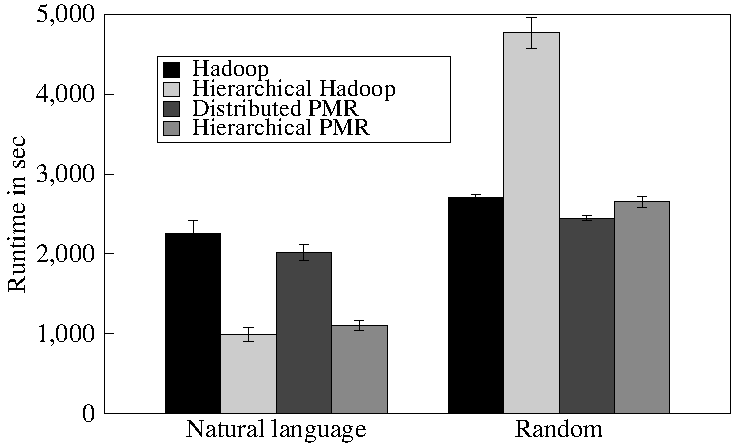
\includegraphics[width=1\textwidth]{figures/allmrs_rands.pdf}
                \caption{}
                \label{fig:allmrs_rands}
        \end{subfigure}

	\caption{Table ~\ref{tab:data-volumes} shows the input, intermediate and output data volumes for WordCount applications on natural language and random data. Figure ~\ref{fig:allmrs_rands} shows WordCount on 16\,GB Data Using Hadoop, Hierarchical Hadoop, Distributed PMR  and Hierarchical PMR}
	\label{fig:combo_1}

\end{figure}




The initial input data of 16\,GB is equally distributed on these two machines. For the single resource Hadoop configuration, half of the input data needs to be moved from
Sierra to Hotel prior to running the actual MapReduce
job.  Figure~\ref{fig:allmrs_rands} shows the results. For natural language
input, both Hadoop and PMR show comparable performance. A major
determinant of performance for Hadoop (in the case of distributed
data) is the necessity to move parts of the data (half of the input
data) to the central Hadoop cluster. The performance of PMR is
determined by the runtime of the map and reduce phase, which are
slightly longer than for Hadoop mainly due to the resource
heterogeneity and the resulting scheduling overhead: the slowest node
determines the overall runtime of both the map and reduce phase.

Both hierarchical Hadoop and PMR perform better than
the distributed PMR and single resource Hadoop configuration. The
performance is mainly influenced by data movement costs. In the
distributed PMR scenario, half of the {\it intermediate} data needs to
be moved to the other resource; in the hierarchical case half of the
{\it output} data requires movement. Since the output data in the
hierarchical case is a magnitude smaller than the intermediate data in
the distributed case (cmp. table~\ref{tab:data-volumes}) -- 20\,MB in
cmp. to 30\,GB -- the performance in the hierarchical case is
significantly better.

For random data, the distributed PMR and single resource Hadoop
perform better than the hierarchical PMR and hierarchical Hadoop
configuration. As the output data is approximately equal to the
intermediate data (30\,GB), i.\,e.\ the advantage of a reduced
transfer volume does not exit. For random data, the additional
MapReduce run represents an overhead. In the Hadoop case, the moved
data needs to be loaded into HDFS, which represents another overhead.



%%%%%%%%%%%%%
%Conclusion
%%%%%%%%%%%%%
%Our experiments show PMR provides the desired flexibility in the deployment and configuration %of MapReduce runs to address specific application characteristics and achieve an optimal %performance, both locally and over wide-area multiple clusters.
Pilot-MapReduce provides a flexible runtime environment for MapReduce applications on general-purpose distributed infrastructures, such as XSEDE~\cite{xsede} and FutureGrid. It brings the advantages of the Pilot abstraction to MapReduce, and enables utilization of federated and heterogeneous compute and data resources. In contrast to Hadoop, no previous cluster setup, which includes running several Hadoop/HDFS daemons, is required. Pilot-MapReduce provides a extensible runtime environment, which allows the flexible usage of sorting in the shuffle, more fine-grained control of data localities and transfer, as well as support for different MapReduce topologies. Using these capabilities, applications with different characteristics, e.g. compute/IO and data aggregation ratios, can be efficiently supported.



\section{Replica Exchange}

Replica-Exchange (RE) methods represent a class of algorithms that involve a large number of loosely-coupled ensembles and are used to understand physical phenomena – ranging from protein folding dynamics to binding affinity calculations. The SAGA-based Pilot Framework, BigJob, has been shown to support this class of applications on FutureGrid as well as XSEDE resources.  There exist two class of RE algorithms namely Synchronous and Asynchronous.  In principle the asynchronous RE algorithm should have better performance in the presence of heterogeneous and distributed resources.

% Synchronous Replica-Exchange:
% Traditionally, RE algorithms have been implemented such that the exchanges have been synchronous.For the synchronous RE formulation, all replicas must reach a pre-determined 
% state before exchanges are performed.All replicas need to finish running before any exchanges are attempted. This synchronization step has the potential to become a serious 
% bottleneck when the ensemble contains large number of replicas. In any implementation, it is highly likely that the coordination of the synchronization step of a large number 
% of replicas will be a costly operation.A major limitation of this model is that the replicas are paired in fixed groups and thus exchanges take place between pre-determined 
% pairs of replicas.But it has an advantage where there is no need to find a replica for pairing, thus eradicating search time.

% Asynchronous Replica-Exchange:
% In the asynchronous RE algorithm, a replica does not have to wait for all other replicas to reach a pre-determined state. An exchange can occur whenever a replica reaches a pre-determined state. The replica then attempts an exchange with any other available replica in the ensemble.Thus, in the asynchronous algorithm, each replica after completing a run has to search and find a new partner is not zero.However waiting time i.e time to synchronize with another pair of replica is zero.In other words, a reduction in synchronization times comes at a cost of increased coordination costs. We do not see an  obvious performance bottleneck in the asynchronous RE.Time for exchange is dependent on the implementation and thus with an efficient implementation we can see a good performance with asynchronous RE even with large number of replicas.

% Replica-Exchange Manager:
% The RE-Manager is the master process which in addition to controlling the different components-SAGA BigJob framework, the individual replicas, etc., also defines and implements the coordination/exchange mechanism employed. The actual tasks that the RE-Manager performs depends not only on the RE algorithm employed, but also on the replica management scheme being supported.The RE-Manager supports two different replica management schemes: centralized and decentralized.In centralized, the RE-Manager manages all the replicas and performs the exchanges.In the decentralized case, a replica-agent manages each replica individually as well making and performing exchange decisions.On Futuregrid, the synchronous and asynchronous RE algorithms were implemented and experiments were run using the centralized RE-Manager.

Experiments and Results:
We have used Futuregrid clusters namely: Sierra, India, Alamo and hotel to run our experiments.We have requested upto 128 cores on all these clusters of Futuregrid. At times due to non-availability of requested resources on future grid ,we have queue times, which we have not included in our total run time of our experiments.Also,not all experiments of Synchronous were run on all machines due to non availability of requested cores. we evaluate and compare the scale-across performance of the algorithms in conjunction with our framework.To understand the scaling behavior of the different RE formulations, we analyze total time to completion (T) for different replica counts from 4, 8, 16, 32. We have kept the ratio of number of attempted exchanges to the number of replicas as constant. The number of times each replica is restarted to complete all exchanges remains constant.Hence the comparison between different cases will reveal differences in coordination cost.The increase is however not uniform between the two 
implementations: it is largest for synchronous RE than Asynchronous RE.We analyzed the total run time on Futuregrid machines and values for all the different replica counts can be seen in the following graph
\begin{figure}[t]
	\centering
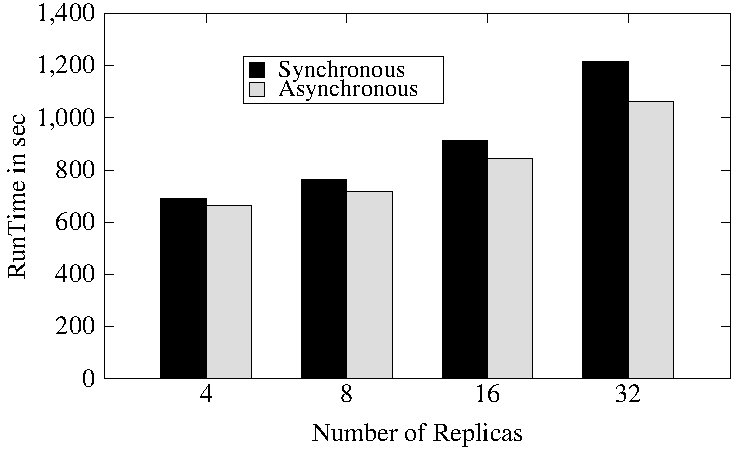
\includegraphics[width=0.47\textwidth]{figures/FG_RE.pdf}
\caption{Centralized Replica-Exchange Mechanism: Synchronous vs Asynchronous} 	
\label{figure(i)}
\end{figure}		

In the above figure(i): As we scale across the number of replicas along with number of machines, keeping number of replicas to number of exchange ratio constant. We can observe that Asynchronous RE outperforms Synchronous RE. This is due to increase in synchronization cost (waiting times) in synchronous RE. Thus, these experiments of RE on Futuregrid clusters demonstrates scalability and interoperability of SAGA-based Pilot Framework, BigJob.

% \mrnote{What do you want to say about this? Abhinav's work?? I am concerned that this overlaps with the fcpc2012-all paper...}

\section{Cactus Spawner}
The Cactus Spawner project envisions application frameworks with simulations that
can be broken down to their constituent components and run across multiple
distributed systems.  A chief consideration is that of ``intelligent computing'',
of knowing when and where to run simulation components separately from the main
simulation.  Work is being done to enable this by modeling simulation components
and predicting the time to run locally vs. the time to transport them and execute
them remotely.  To model real-world problems, the Cactus framework is used, and
actual black hole simulations are executed and spawned from.  Contributions
to the field involve algorithms in modeling, spawning, and performance evaluation on
the I/O systems of FutureGrid hardware.  Of special note is the role SAGA plays in the
Spawner project; SAGA allows multiple middleware systems to be specified without the need
for extensive code rewriting to support each middleware.

FutureGrid resources were key to the initial development of the Spawner technology.
HPC resources \textit{Alamo} and \textit{Hotel} were used to develop the methods of separating functions
from the main simulation. Details of the Spawner
mechanism developed on FutureGrid can be seen in figure~\ref{fig:spawner}.
The large scale needed to run the spawning experiments precluded the use
of FutureGrid hardware for the main simulation runs.   For this reason, simulation results were gathered
on XSEDE machines.  The base research behind the Spawner technology
was still conducted on FutureGrid, including the initial coding and testing.  

\begin{figure}[t]
	\centering
		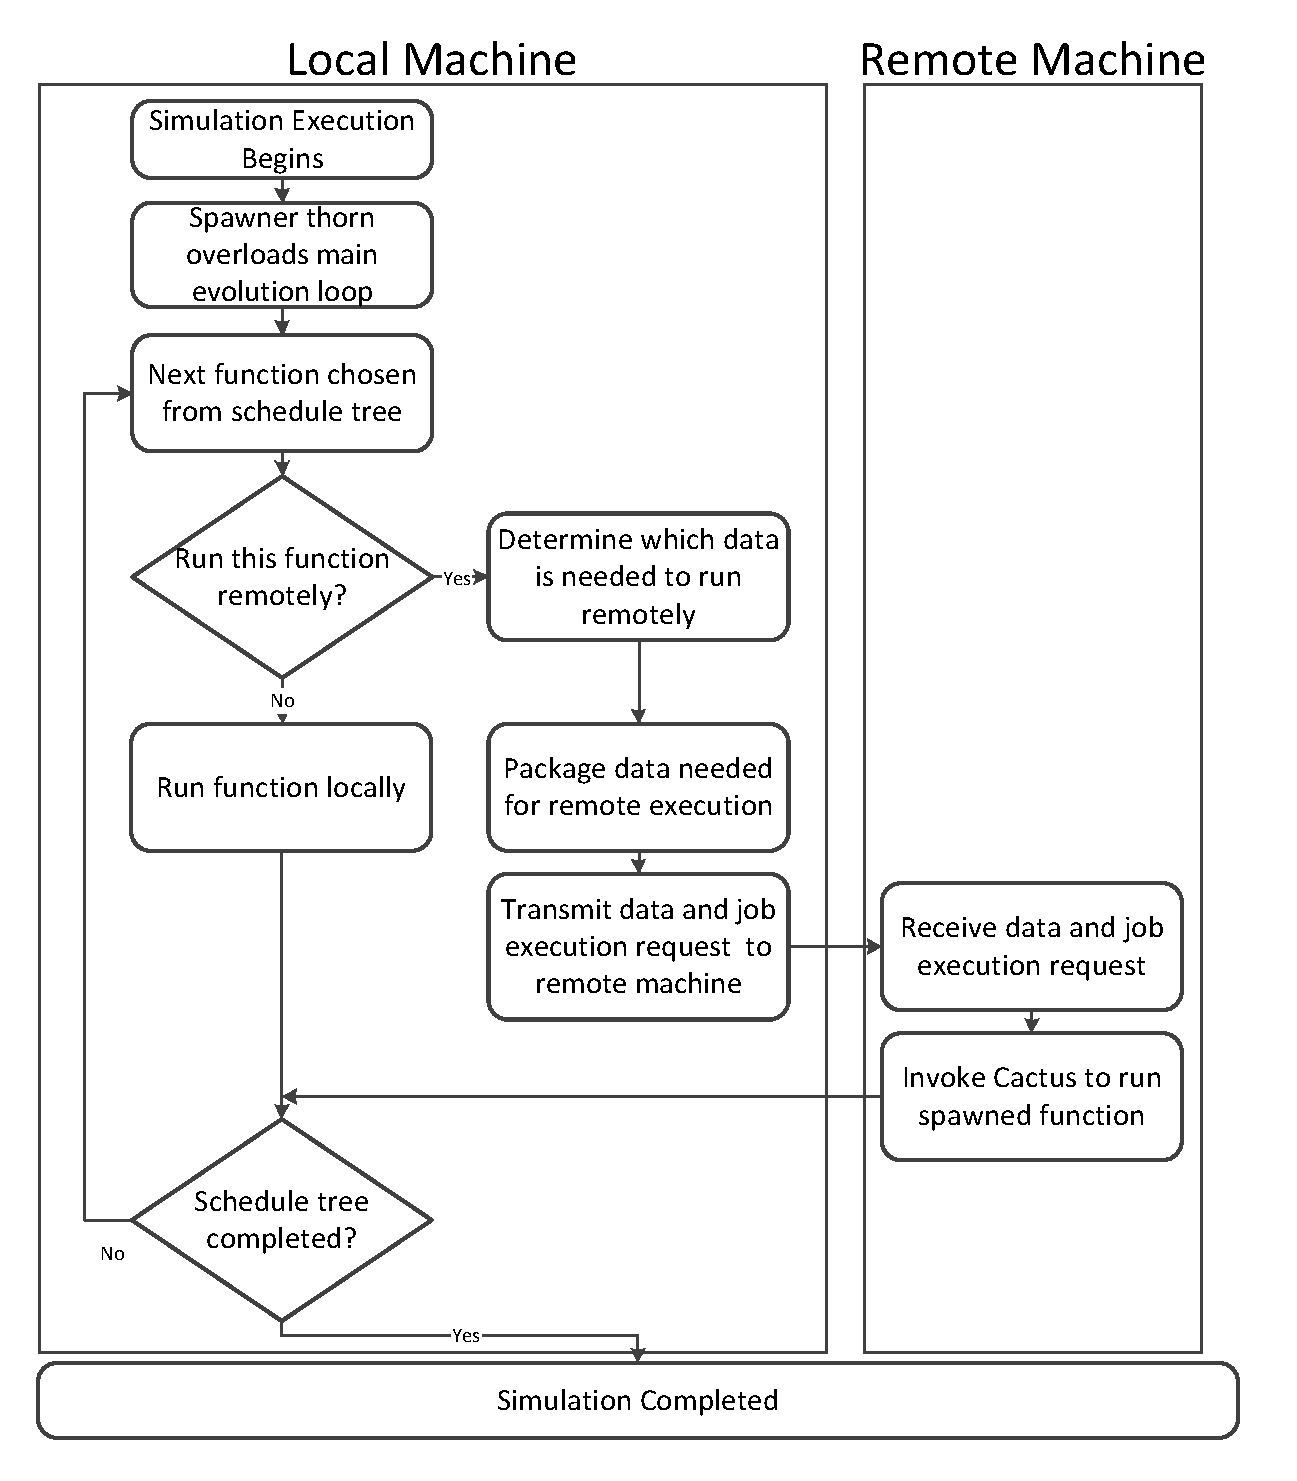
\includegraphics[width=0.40\textwidth]{figures/spawner-logic.pdf}
\caption{Spawner decision-making logic}
\label{fig:spawner}
\end{figure}		

The eventual goal of the Spawner project is to provide a basis for an increase in
scalability and interoperability for future simulation frameworks.  An increase in scalability
may be realized by executing nondependent functions in parallel across multiple machines rather
than in serial on one.  An improvement in interoperability may be realized by making use of heterogeneous systems,
enabling simulation functions to run on the machines which suit them best.  This is naturally improved through
the use of SAGA, which extends the range of systems which may be utilized.  With SAGA and the
selective execution technology behind Spawner, both scalability and interoperability between systems
can be enhanced.

\section{SAGA-Bliss Development} SAGA-Bliss is an implementation of the OGF
GFD.90 SAGA standard, built with an emphasis on usability and ease of
deployment.  To this end, it makes use of Python and a less-than-strict
adherence to feature completeness or standards obedience.  In short, the focus
of the SAGA-Bliss implementation is to have a highly-usable API for distributed
computing with a low barrier of entry for application development. The
SAGA-Bliss code base is still under heavy initial development, and FutureGrid
was found to be an ideal location for development and testing.

Two key features for SAGA-Bliss were developed while making use of FutureGrid resources; 
the SSH and Eucalyptus cloud plugins.  The SSH plugin enables the use of the SSH protocol
to submit jobs to remote resources, utilizing SAGA abstractions such as contexts in order
to specify authentication information.  The Eucalyptus plugin allows users to access
Eucalyptus compute clouds, starting up, shutting down, and querying virtual machines.
Adding these additional plugins to SAGA-Bliss contributes greatly to the interoperability of
SAGA-Bliss, with each new plugin providing a means of communicating with a new resource.

Initial results on FutureGrid's \textit{India} and \textit{Sierra} indicate
that the SSH plugin works and is useful for cross-machine job submission, and
indeed the SSH plugin passes all SAGA-Bliss job plugin test cases.  The
Eucalyptus plugin is successful starting, stopping, and querying virtual
machines.  To test the functionality of the plugins together, a scenario of
cloud resources running Cactus simulations was developed.  From within
SAGA-Bliss, first a virtual machine is booted, then a Cactus job is sent to the
virtual machine and successfully executed, the remote machine terminating once
execution has completed.  This proves that the SAGA-Bliss approach maps well to
handling cloud compute resources, and that scientific simulations can be
executed successfully from this base.  Continued development on SAGA-Bliss will
increase the degree of interoperability that SAGA-Bliss offers between
distributed resources, with additional plugins offering additional methods of
communicating with resources in much the same way the SSH and Eucalyptus
plugins offer access to SSH servers and Eucalyptus compute clouds.

%As Bliss is developed further, achieving a high degree of interoperability
%between distributed systems will be as simple as choosing between the systems a user would like
%to access, letting plugins like the SSH plugin and the Eucalyptus plugin handle the rest.

\section{Production Infrastructure: Deployment and Testing}

SAGA and BigJob are deployed~\cite{saga-depl} on all major FutureGrid machines (India,
Sierra, Hotel and Alamo).  FutureGrid provides Community Software
Areas (CSA) to communities, which basically is a system level area
where software packages can be shared among a community of users.
While it is possible to install and use SAGA and BigJob in each user's
directory, to ensure minimum repetition of effort and to ensure users
of SAGA get the best possible support, we employ the CSA model.  It is
not the case that SAGA per se is difficult to install, but the fact
remains that the adaptors to the many middlewares have widely varying
configuration and deployment requirements.  Thus having a central
location on each machine where SAGA is deployed as a community code
ensures effective and correct installation.  Similar considerations
hold for Bigjob and SAGA-Bliss -- it was therefore only logical to deploy
SAGA and BigJob in a CSA space on FutureGrid machines.

The source code for SAGA, BigJob and SAGA-Bliss is stored in a git
repository~\cite{saga-github}, and the deployment scripts pull sources
from specific branches in the repository.  A set of semi-automatic
deployment scripts is used to manually trigger CSA software updates.
An update can encompass an individual machine or all machines, an
individual SAGA component or the entire SAGA/BigJob/SAGA-Bliss stack. The
set of supported components includes the SAGA core libraries,
different API packages, the supported middleware adaptors for each
machine, the python bindings, and the BigJob package and its
dependencies, and SAGA-Bliss. 

The CSA installations are accompanied by automatically generated
documentation (READMEs) and configuration scripts, which simplify the
environment settings for the end user.  Site specific configuration
details are also documented on github wiki pages.  For BigJob, a
github wiki is used to store user guides for each of the individual
FutureGrid machines. 

A BigJob CSA release is the result of a testing and deployment
pipeline. Any newly developed features, code modifications and bug
fixes are created in branches and are later merged onto the master.
Once merged, it is deployed as experimental feature.  After each
update, a set of manual tests is performed to ensure the validity of
the deployment candidate.
% automated unit tests are automatically run on the target machines,
% which includes test suite downloaded from SVN at runtime.  Test
% results are later committed back to a common repository.  By doing
% this we ensure that not only the updated version is deployed, but
% more importantly, that it is correctly installed and configured for
% that target machine. The unit tests range from basic (low-level)
% environment testing, to application level test runs of a BigJob
% application. The user can also submit own scripts by passing the
% location of the script as a argument to the test script.  README,
% module file and test results are all committed to the central SAGA
% code repository~\cite{r_link}, and (partially) used to document the
% current state of deployment on the SAGA deployment wiki. 
%
After testing is complete, the python code is (manually) pushed to the
Python Package Index (\textit{pypi}). This code is then deployed into
the CSA space using pypi. Careful consideration is taken to ensure
that the updates to CSA space will not impact any current users of
BigJob on the target resources. Another round of testing is then
completed to verify that the CSA installations are working and no
changes to the users' environments are required.  The deployment
documentation (README), a generated 'module' file and basic test
results are all committed to the central SAGA code
repository~\cite{saga-test}, and (partially) used to document the current
state of deployment on the SAGA deployment wiki.  Any corresponding
documentation on the BigJob github wiki is updated to reflect the
changes.

For SAGA and for SAGA-Bliss, an additional set of tests are running after
the CSA deployment completed, ti verify the viability of the
installations.  For SAGA, those tests are relatively simple, and check
if the expected set of adaptors are available and load correctly.  For
SAGA-Bliss, the set of tests is more elaborate, and also cover correct
environment settings, and n:m testing of remote system access: for
example, a test run for the SAGA-Bliss installation on India would attempt
to submit test jobs via ssh and pbs+ssh to Alamo, Sierra and Hotel.
As those tests use exactly the environment settings which are
documented for the end user, we gain some confidence that the
installation is in fact viable.  Test results are timestamped and
again pushed back into the SAGA git repository.

Additionally, SAGA-Bliss is using another buildbot~\cite{bliss-buildbot}
driven test regime to ensure the stability of the SAGA-Bliss code base in
respect to FutureGrid and XSEDE as target environments: on every git
code update (and also at regular intervals), a set of tests is run on
all FutureGrid backends, to verify that the SAGA-Bliss master branch is in
usable state, and to notify the developers of potential problems as
early as possible.  That mechanism proves extremely valuable for the
release process of SAGA-Bliss.


\section{SAGA and BigJob on FutureGrid Cloud Resources}

Though SAGA was originally developed for Grids and clusters, its importance must also be considered in the context of Cloud computing. SAGA for Clouds provides a promising route for cloud-cloud and cloud-grid interoperability, in addition to providing a useful and consistent set of abstractions for compute and data management across grids and clouds.

SAGA on clouds has been used to provide %the overall goal of achieving the 
``distributed functionality'' for data-intensive applications. Grids and Clouds differ in many semantical aspects, such as service-based vs. direct resource access, what scalability entails, and differences in platforms. SAGA requires functionality that allows the application to be immune to the fact that it is running on a Grid vs. a Cloud. This functionality is achieved through a context-aware adaptor that is dynamically loaded. Interoperability at the application-level must be provided through the use of such adaptors. SAGA on clouds facilitated the development of a Eucalyptus adaptor to spawn the virtual machines. The ssh adaptor was used to submit jobs to the actual machines. 
st
The natural extension of this work is to try to use BigJob, the SAGA-based Pilot Job framework, with clouds. BigJob has been shown in the past to work with both the Windows Azure Cloud operating system and Nimbus platform. On FutureGrid, cloud capabilities are offered through a choice of Iaas platforms -- Eucalyptus, Nimbus, or OpenStack. Testing of SAGA and BigJob on Cloud resources was performed on India with both Eucalyptus and OpenStack. Though SAGA had been tested with both Eucalyptus and Nimbus before, it had yet to be tested on the new OpenStack resources on India. India offers both OpenStack Nova (compute resources) and Swift (storage). Preliminary work on integrating SAGA with these resources focuses only on Nova and job submission, but in the future, the focus will shift to cloud-based storage to support both scalability and data exchanges.

Much of the continued efforts on FutureGrid will be to adapt BigJob to be able to spin up as many VMs as it needs for a given pilot-job based on the number of jobs and the number of cores required for those jobs. The existing BigJob functionality of an agent that submits subjobs to different ``machines'' can be leveraged and applied to the cloud environment (in this case, the machines would be the public IP addresses of the VMs that were spun up using BigJob). To achieve this, the SAGA-Bliss Eucalyptus adaptor will be integrated with the BigJob API. The Eucalyptus adaptor can be used to create the virtual machines, shut them down, and query their statuses. The context-aware adaptor is still necessary for providing the private key for each virtual machine in order to have the authorization to submit jobs via ssh.

Once this integration is complete, performance of Grids vs. Clouds on FutureGrid can be evaluated. The scientific applications that are best suited to utilize BigJob for Clouds can also be investigated, in addition to interoperability tests. There may be times when it makes sense to utilize both Clouds and Grids based on the given application, and this work can help to identify when it is appropriate. Lastly, BigJob will be shown to work with Eucalyptus, Nimbus, and OpenStack, thus providing capabilities to submit to all of the IaaS platforms that FutureGrid provides.


\section{Conclusion}
Here we will evaluate each application based on how they fit into the
FutureGrid proposal criteria.
\begin{enumerate}
\item Interoperability
\item Scalability
\item Contribution to Education
\item Research (innovation, quality of papers, new software, algorithms, insightful performance measurements, etc.)
\end{enumerate}

\bibliographystyle{plain}
\bibliography{pilotjob,saga,saga-related,mrbib}

\end{document}
